\documentclass[11pt]{article}
\usepackage[a4paper,margin=22mm,headheight=16pt]{geometry}
\usepackage{fontspec,xeCJK,xcolor,graphicx,enumitem,fancyhdr,titlesec}
\usepackage{hyperref}
\IfFontExistsTF{Times New Roman}{\setmainfont{Times New Roman}}{\setmainfont{TeX Gyre Termes}}
\IfFontExistsTF{FangSong}{\setCJKmainfont[AutoFakeBold=2]{FangSong}}{\IfFontExistsTF{仿宋}{\setCJKmainfont[AutoFakeBold=2]{仿宋}}{\IfFontExistsTF{FandolFang-Regular.otf}{\setCJKmainfont[AutoFakeBold=2]{FandolFang-Regular.otf}}{\setCJKmainfont{FandolSong-Regular.otf}}}}
\definecolor{ink}{HTML}{173747}\definecolor{accent}{HTML}{227E82}
\hypersetup{colorlinks=true,urlcolor=accent,linkcolor=accent}
\linespread{1.22}\setlength{\parindent}{0pt}\setlength{\parskip}{6pt}
\setlist[itemize]{leftmargin=1.4em,itemsep=3pt}
\titleformat{\section}{\large\bfseries\color{ink}}{}{0pt}{}
\titlespacing*{\section}{0pt}{14pt}{7pt}
\pagestyle{fancy}\fancyhf{}\lhead{\small OMNI LEARNING / 学习手册}\rhead{\small Source-grounded learning}\cfoot{\small\thepage}
\emergencystretch=2em\widowpenalty=10000\clubpenalty=10000
\newcommand{\Needspace}[1]{\par\begingroup\dimen0=#1\relax\vskip0pt plus\dimen0\penalty-100\vskip0pt plus-\dimen0\vskip\dimen0\penalty9999\vskip-\dimen0\vskip0pt\endgroup}
\begin{document}


{\LARGE\bfseries\color{ink} 节拍节奏与速度}\par

2026-10-08 | Day02/30 | 阅读 8 分钟 + 练习 3 分钟\par\vspace{6pt}

\Needspace{5\baselineskip}\section*{今日导航}

今天回答：跟着歌打拍子，是否等于跟着所有音符？目标是把稳定脉冲、具体节奏和快慢区分开。先回忆昨天：同一节奏可以用不同音高、不同力度演奏，这意味着时间组织值得单独观察。

\Needspace{5\baselineskip}\section*{用身体找到时间参照}

均匀地轻拍桌面八次，把它当作参照脉冲。保持轻拍，嘴里念一句熟悉的短句：字不一定恰好落在每次拍击上，也可能一拍里有两个字或没有字。这里用日常语言做教学类比，不意味着说话天然符合某一种音乐拍号。

节奏指声音与停顿在时间中的具体组织；节拍提供组织和预期。公开乐理教材把音符时值与休止分开标记，提醒我们停顿也是时间结构的一部分。[S3]

\begin{center}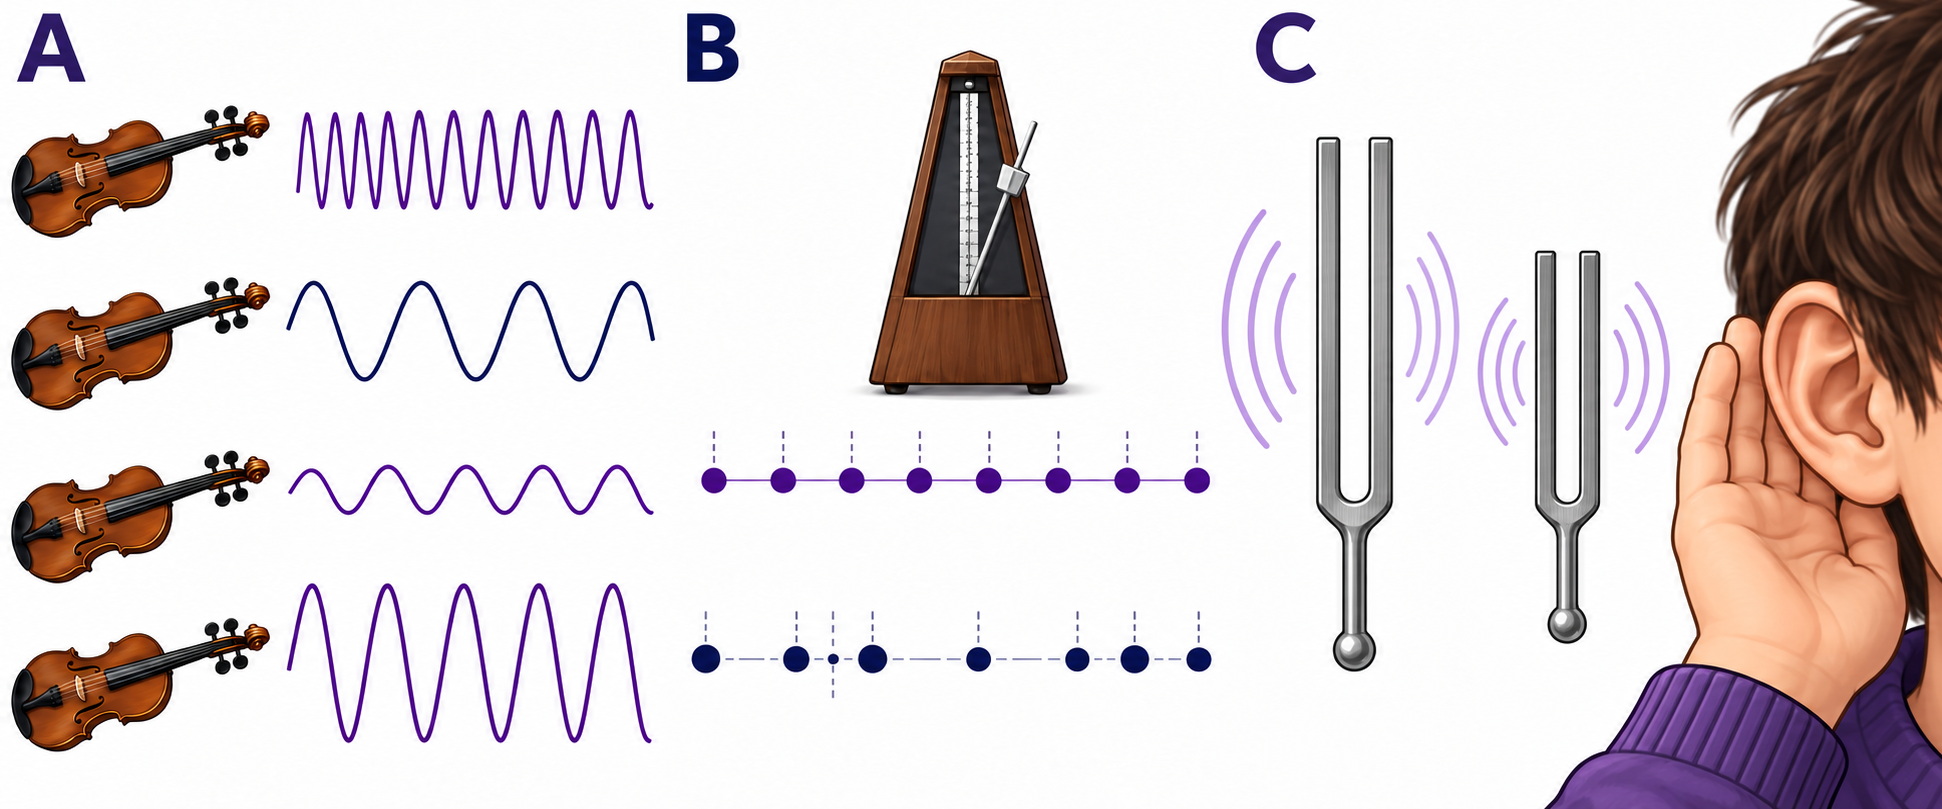
\includegraphics[width=\linewidth,height=0.26\textheight,keepaspectratio]{../assets/figure-f6141a0bb6d5.png}\par

{\small 本课重点看 B 区。A 比较振动疏密与振幅；B 稳定脉冲和节奏事件并不相同；C 两个音高之间可以比较方向与距离。波形仅作概念示意。}\par

{\footnotesize AI生成教学示意，非实物照片、原始史料或官方架构。生成方式：内置文生图；提示词见仓库 docs/image-prompts.json。}\end{center}

\Needspace{5\baselineskip}\section*{拍子分组与速度}

速度描述脉冲进行的快慢。拍子分组则描述你怎样感到周期性的重心，例如两拍或三拍一组。二者可以独立：三拍子的音乐既可能缓慢，也可能轻快。教材讨论西方常见节拍时，还区分每拍二分或三分的方式；这些属于进一步的结构，不是今天必须背下的全部分类。[S4]

不要从“听起来很快”直接推断拍号。音符很密而基本拍速不变，也会显得忙碌。反过来，拍子较快但长音很多，表层可能显得平稳。遇到自由节奏、复杂重音或不熟悉的传统时，允许先说“我暂时没有找到稳定参照”，而不是强行数成四拍。

\Needspace{5\baselineskip}\section*{图 B：同一条时间线上两种事件}

图 B 上排点等间隔，表示稳定参照；下排事件不等间隔，表示具体节奏。先沿上排点轻拍，再试着在下排点位置发声。重点是让脚下或手上的脉冲继续，而不是每出现一个声音就改变拍速。

教学设例：在四个均匀拍点中，第一拍发声，第二拍发两次短声，第三拍静默，第四拍发声。总共仍是四拍，声音事件数却不是四。若把“事件数量”等同于“拍数”，你会越数越乱。实际作品中的停顿并不意味着内在脉冲一定消失。

\Needspace{5\baselineskip}\section*{三分钟练习与自查}

先均匀拍八次；然后每两拍把第一拍拍得稍重，最后改成每三拍一组，允许最后一组不完整。保持拍速大致相同。再回答：你改变的是速度还是分组？

参考：主要改变分组。若每组都想在同样时间内完成，就会无意改变拍速；重新用连续均匀的拍点检查。可选读 [S4] 中的聆听示例，不要求今天打开所有播放器；若访问受限，用本页身体练习也能完成目标。

\Needspace{5\baselineskip}\section*{复盘与明日连接}

节拍是参照与组织，节奏是具体事件，速度是快慢。三者相互关联，却不能互相替代。明天把时间与高低结合起来：为什么不同起点的一段旋律仍可能被认作同一首歌？

\Needspace{6\baselineskip}\section*{扩展学习 / Further reading}\small 以下为选读，不计入每日必做时间。\begin{enumerate}[leftmargin=1.6em]

\item [S1] \href{https://openstax.org/books/physics/pages/14-1-speed-of-sound-frequency-and-wavelength}{Speed of Sound, Frequency, and Wavelength} — 选读声音频率与音高的关系，公式推导可跳过。\par OpenStax | 发布：未标注 | 核验：2026-10-08

\item [S2] \href{https://openmusictheory.github.io/basicNotation.html}{Basic notation} — 认识音符、谱表和变音记号；本课不要求记住全部符号。\par Open Music Theory | 发布：未标注 | 核验：2026-10-08

\item [S3] \href{https://openmusictheory.github.io/rhythmicValues.html}{Rhythmic values} — 观察长短时值和休止符如何表达时间。\par Open Music Theory | 发布：未标注 | 核验：2026-10-08

\item [S4] \href{https://openmusictheory.github.io/meter.html}{Meter and time signatures} — 选看拍子分组与聆听示例；部分嵌入播放器可能需要额外登录。\par Open Music Theory | 发布：未标注 | 核验：2026-10-08

\item [S5] \href{https://openmusictheory.github.io/intervals.html}{Intervals and dyads} — 重点看半音数与音程度数不是同一种计数方法。\par Open Music Theory | 发布：未标注 | 核验：2026-10-08

\end{enumerate}

\end{document}